\documentclass{article}
\usepackage{cite, hyperref}

\title{contiBAIT: Improving Genome Assemblies Using Strand-seq Data}
\author{Kieran O'Neill, Mark Hills and Mike Gottlieb}

%\VignetteIndexEntry{flowBi}ngit 

\usepackage{Sweave}
\begin{document}
\Sconcordance{concordance:contiBAIT.tex:/data/ContiBAIT/vignettes/contiBAIT.Rnw:%
1 8 1 1 0 31 1 1 4 3 0 1 4 3 0 1 3 4 0 1 2 2 1 1 3 11 0 1 4 2 0 2 1 3 0 %
1 2 4 1 1 4 6 0 1 2 4 1 1 4 3 0 1 1 6 0 1 2 5 1 1 2 1 0 1 1 2 2 2 1 1 2 %
10 0 1 1 15 0 1 2 2 1 1 2 4 0 1 2 6 1}

\setkeys{Gin}{width=0.65\textwidth}
\setkeys{Gin}{height=0.65\textwidth}

\maketitle
\begin{center}
{\tt koneill@bcgsc.ca}
\end{center}

\textnormal{\normalfont}

\tableofcontents
\newpage

\section{Licensing}
Under the Two-Clause BSD License, you are free to use and redistribute this software.

\section{Introduction}
Strand-seq is a method for determining template strand inheritance in single cells.
When strand-seq data are collected for many cells from the same organism, spatially close genomic regions show similar patterns of template strand inheritance.
ContiBAIT allows users to leverage this property to carry out three tasks to improve draft genomes.
Firstly, in assemblies made up entirely of contigs or scaffolds not yet assigned to chromosomes, these contigs can be clustered into chromosomes.
Secondly, in assemblies wherein scaffolds have been assigned to chromosomes, but not yet placed on those chromosomes, those scaffolds can be placed in order relative to each other. Thirdly, for assemblies at the chromosome stage, where scaffolds are ordered and separated by many unbridged sequence gaps, the orientation of these sequence gaps can be found.  

All three of these tasks can be run in parallel, taking contig-stage assemblies and ordering all fragments first to chromosomes, then within chromosomes while simultaneously determining the relative orientation of each fragment.

%\section{Correcting misorientations within scaffolds} %coming soon
\section{Input}
ContiBAIT requires input in BAM format. Multiple BAM files are required for analysis, so ContiBAIT specifically calls for users to identify a BAM directory in which to analyse. BAM files should be sorted prior to analysis.
To read in BAM files into ContiBAIT, create a strandFreqTable instance by calling strandSeqFreq 

<<strandSeqFreqTable.R>>

\section{Assigning contigs or scaffolds to chromosomes}

\begin{Schunk}
\begin{Sinput}
> #Loading
> library(contiBAIT)
> plot(hist(rnorm(1000)))
\end{Sinput}
\end{Schunk}
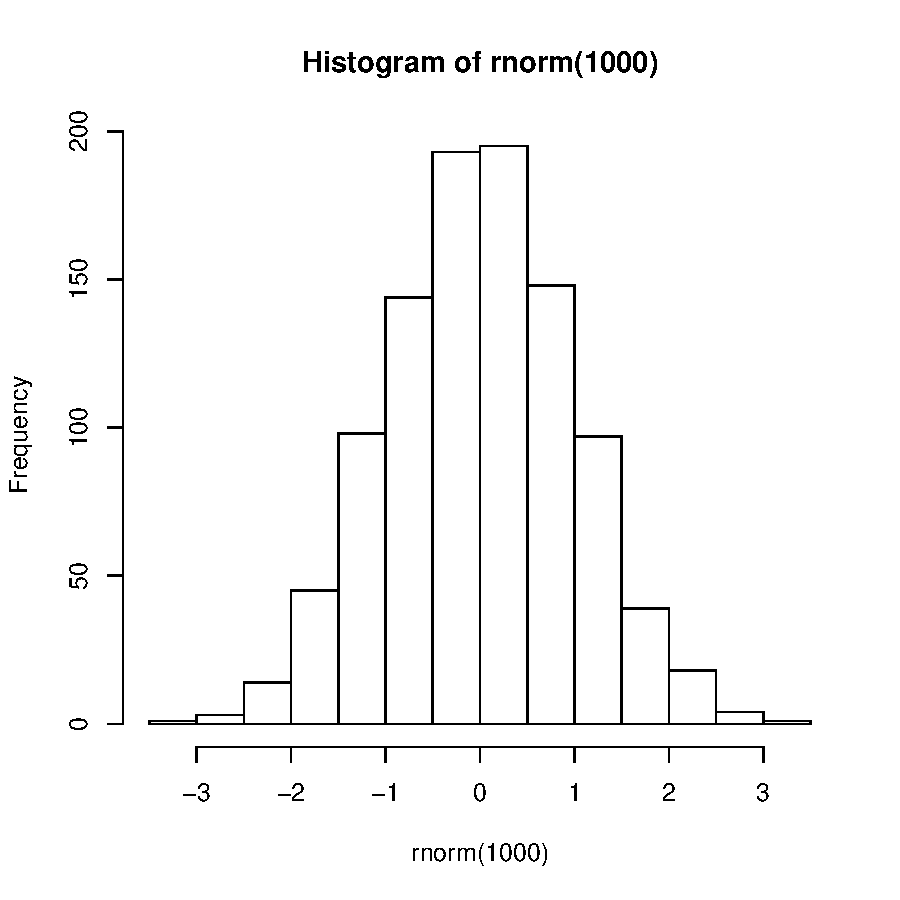
\includegraphics{contiBAIT-examplea}


\section{Ordering contigs or scaffolds within chromosomes}
First we load our artificial murine chromosome data. Some words about the meaning of linkage.group, animal.tab, and reorientedTable or whatever it's called.
\begin{Schunk}
\begin{Sinput}
> #   data(contigOrderingExample)
> #   reorientedTable <-  vignetteTestData[[1]]
> #   animal.tab <- vignetteTestData[[2]][[1]]
> #   linkage.group <- vignetteTestData[[3]][[1]]
> #   set.seed(666)
\end{Sinput}
\end{Schunk}
Next we sort the artificial mouse contigs using contiBAIT.
\begin{Schunk}
\begin{Sinput}
>   ordering <- 'ordering'
\end{Sinput}
\end{Schunk}
The resulting ordering can then be plotted.

\section{Writing out to a BED file}
This file can be passed to bedtools along with the original (draft) reference genome to create a new FASTA file containing the assembled genome.


\end{document}
